\documentclass{standalone}
\usepackage{tikz}
\tikzset{ block/.style = {draw, fill=white, very thick, rectangle, minimum height=1cm, minimum width=2cm},}
\begin{document}
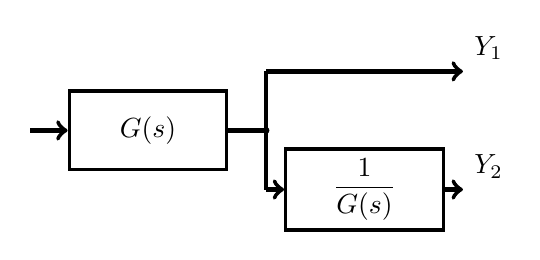
\begin{tikzpicture}
    \node[block](g){$\displaystyle\frac{1}{G(s)}$};
    \draw[-,ultra thick](-1.5,0.75)--(-1.25,0.75);
    \filldraw[black](-1.25,0.75)circle(1pt);
    \coordinate(o)at(-1.25,0.75);
    \draw[-,ultra thick](-1.25,0.75)--(-1.25,0);
    \draw[->,ultra thick](-1.25,0)--(g.180);
    \draw[->,ultra thick](g.0)--(1.25,0)node[above right]{$Y_2$};
    \draw[-,ultra thick](-1.25,0.75)--(-1.25,1.5);
    \draw[->,ultra thick](-1.25,1.5)--(1.25,1.5)node[above right]{$Y_1$}; 
    \node[block, left of=o,node distance=1.5cm](g2){$G(s)$};
    \draw[-,ultra thick](g2.0)--(o);
    \draw[<-,ultra thick](g2.180)--(-4.25,0.75);
\end{tikzpicture}
\end{document}